\section{Alternative Designs}
\label{sect:alternative_designs}

Shown below are two alternative designs that were considered for PyBank but ultimately were discarded for their counterparts which were shown in Section~\ref{sect:static_interface_design}. The first design shown below in Figure~\ref{fig:alt_sign_in_diagram} displays an alternative Sign-in window and the second design also shown below in Figure~\ref{fig:alt_visualization_diagram} displays an alternative checking account visualization window.

\subsection{Alternative Sign-in Window}
\label{sect:alt_sign_in}

The alternative sign-in window displayed below in Figure~\ref{fig:alt_sign_in_diagram} was not chosen for several reasons including the following: the avatar shown in the window should not be placed at the login before the user is known, the window's navigation menu and title do not have a color scheme that helps contrast the bright text colors, and some common window functions (minimizing/maximizing) are also absent from the design. For these reasons, the sign-in window presented in Section~\ref{sect:static_interface_design}, Figure~\ref{fig:signin} was chosen. 

\begin{figure}[H]
	\begin{centering}
	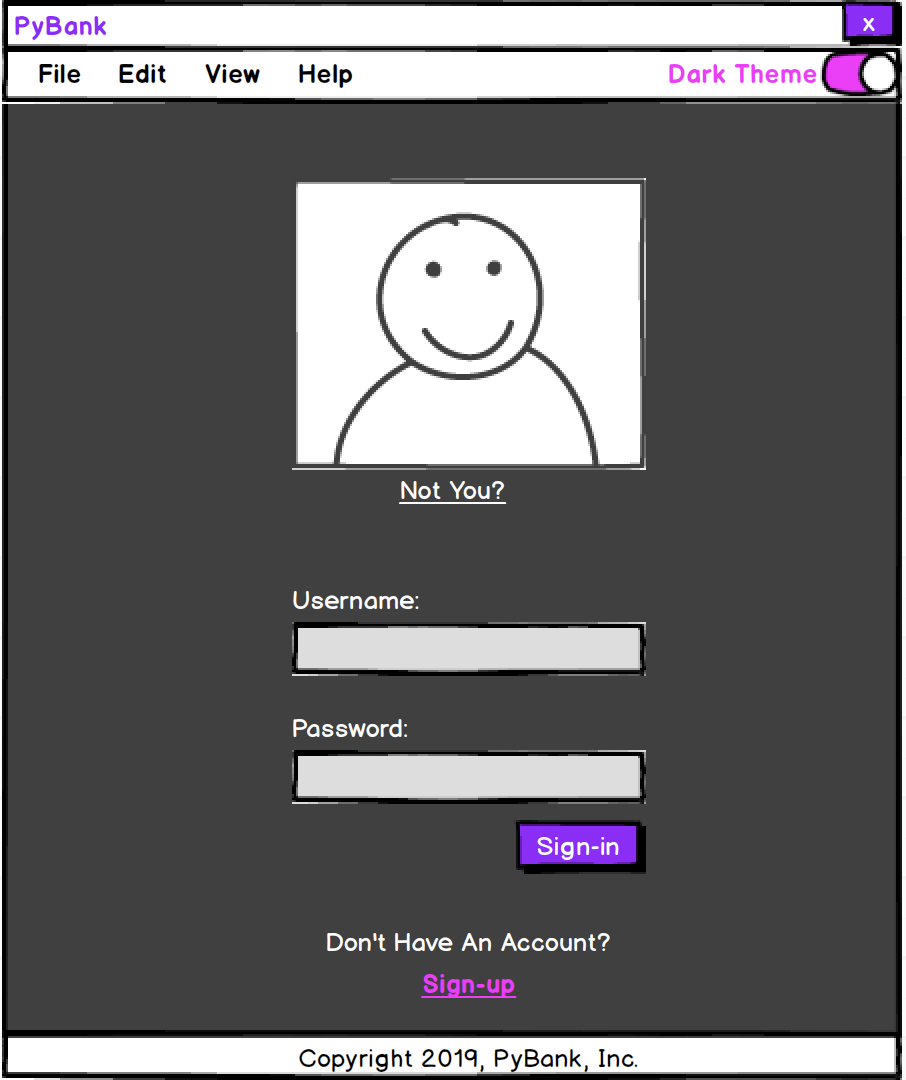
\includegraphics[width=0.55\linewidth, height=0.70\linewidth]{figures/alternative_sign_in_design.png}
	\caption{A medium-fidelity prototype alternative for the sign-in window.}
	\label{fig:alt_sign_in_diagram}
	\end{centering}
\end{figure}

\newpage

\subsection{Alternative Visualization Window}
\label{sect:alt_visualization}

The alternative visualization window for checking accounts shown below in Figure~\ref{fig:alt_visualization_diagram} was not selected for PyBank because it does not provide the user with a wide selection of options. The visualizations presented in the alternative design are limited to \emph{spending vs. time} analysis whereas the chosen design provides radio buttons with multiple criteria that a customer can look at. Other reasons for dismissing this design are similar to the alternative sign-in window where the window's navigation menu and title do not have a color scheme that helps contrast the bright text colors, and some common window functions (minimizing/maximizing) are also absent from the design. For these reasons, the visualization window presented in Section~\ref{sect:static_interface_design}, Figure~\ref{fig:graphs} was chosen.

\begin{figure}[H]
	\begin{centering}
	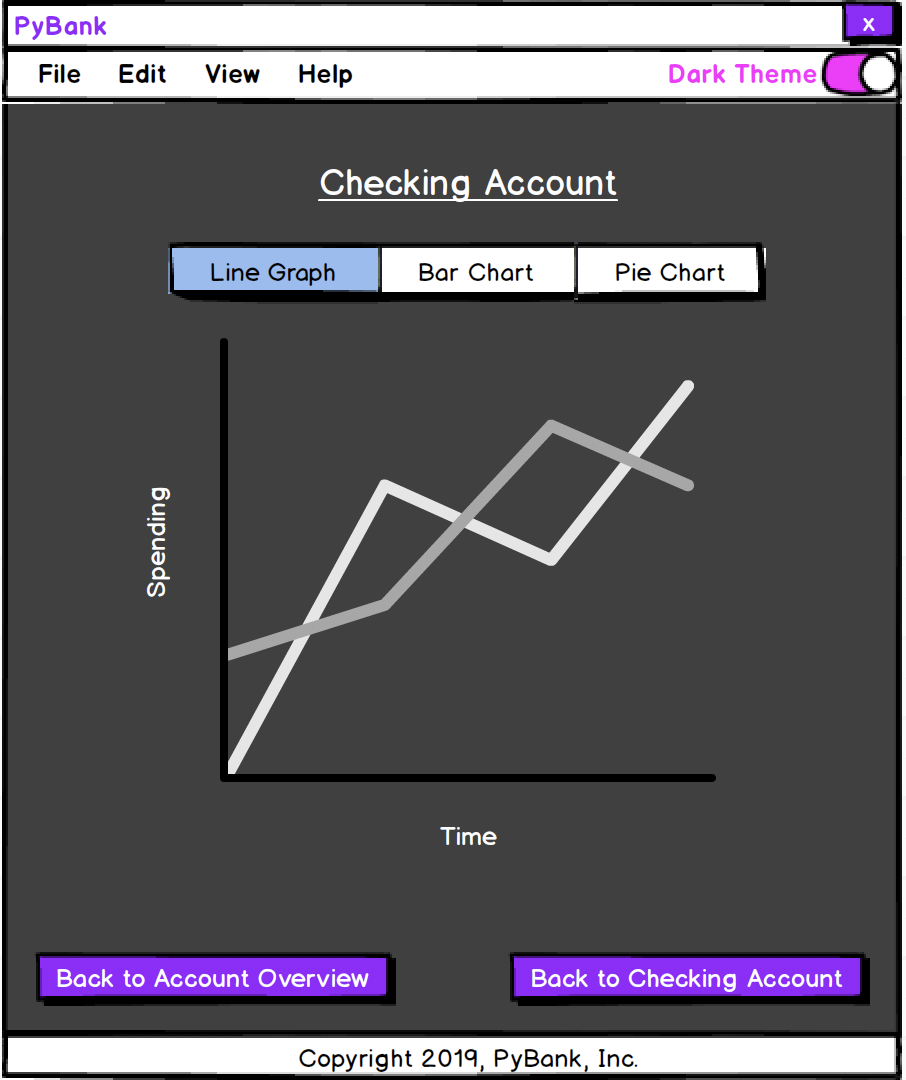
\includegraphics[width=0.55\linewidth, height=0.70\linewidth]{figures/alternative_visualization_design.png}
	\caption{A medium-fidelity prototype alternative for the checking account visualizations window.}
	\label{fig:alt_visualization_diagram}
	\end{centering}
\end{figure}

%EOF